% HMC Math dept HW template example
% v0.04 by Eric J. Malm, 10 Mar 2005
\documentclass[12pt,letterpaper,boxed,cm]{hmcpset}

% set 1-inch margins in the document
\usepackage[margin=1in]{geometry}
\usepackage{mathtools}
\usepackage{mathrsfs}
% include this if you want to import graphics files with /includegraphics
\usepackage{graphicx}
\usepackage{cases}
\usepackage{hyperref}
\usepackage{siunitx}
\usepackage{tikz}
\usetikzlibrary{arrows}

% info for header block in upper right hand corner
\name{Name: ~~~~~~~~~~~~~~~~~~~~~~}
\class{Physics 51}
\assignment{Homework \#2}
\duedate{September 5, 2016}

\newcommand{\ev}[2]{\Big|_{#1}^{#2}}
\newcommand{\evv}[2]{\Big|_{#1}^{#2}}
\newcommand{\set}[1]{\left\{#1\right\}}
\newcommand{\s}[1]{\sqrt{#1}}
\newcommand{\f}[2]{\frac{#1}{#2}}
\newcommand{\p}[2]{\frac{\partial #1}{\partial #2}}
\providecommand{\t}[1]{\text{#1}}
\providecommand{\span}[1]{\text{span}\left(#1\right)}
\providecommand{\set}[1]{\left\{#1\right\}}
\providecommand{\l}[0]{\left}
\providecommand{\r}[0]{\right}
\newcommand{\m}[1]{\begin{matrix}#1\end{matrix}}
\newcommand{\bm}[1]{\begin{bmatrix}#1\end{bmatrix}}
\renewcommand{\bf}[1]{\mathbf{#1}}
\newcommand{\pn}[1]{\left( #1 \right)}
\newcommand{\abs}[1]{\left| #1 \right|}
\newcommand{\bk}[1]{\left[ #1 \right]}
\newcommand{\cis}[1]{\pn{\cos\pn{#1} + i\sin\pn{#1}}}
\newcommand{\cisi}[1]{\pn{\cos\pn{#1} - i\sin\pn{#1}}}
\renewcommand{\Im}[1]{\text{Im}\pn{#1}}
\renewcommand{\Re}[1]{\text{Re}\pn{#1}}

\makeatletter
\renewcommand*\env@matrix[1][*\c@MaxMatrixCols c]{%
  \hskip -\arraycolsep
  \let\@ifnextchar\new@ifnextchar
  \array{#1}}
\makeatother
\begin{document}
\problemlist{25-P4, 26-E16, 26-P2, 25-P7*}

\begin{problem}[25-P4]
  Two Similar tiny balls of mass $m$ are hung from silk threads of length $L$
  and carry equal charges $q$ as in Fig. 14. Assume that $\theta$ is so small
  that $\tan\theta$ can be replaced by its approximate equal, $\sin\theta$.
  \begin{enumerate}
    \item[(a)] To this approximation show that, for equilibrium,
  \[
    x = \pn{\f{q^2L}{2\pi\epsilon_0mg}}^{1/3},
  \]
  where $x$ is the separation between the balls.
  \item[(b)] If $L = \SI{122}{\cm}$, $m =
  \SI{11.2}{g}$, and $x = \SI{4.70}{\cm}$, what is the value of $q$?
  \end{enumerate}
  \begin{center}
    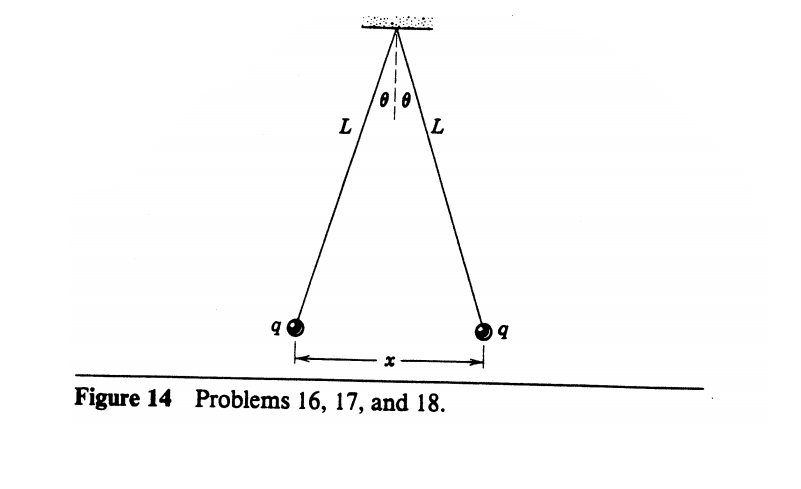
\includegraphics[scale=0.7]{01.png}
  \end{center}
\end{problem}
\begin{solution}
\end{solution}
\newpage

\begin{problem}[26-E16]
  A thin glass rod is bent into a semicircular of radius $r$. A charge $+q$
  is uniformly distributed along the upper half and a charge $-q$ is uniformly
  distributed along the lower half, as shown in Fig. 26-28. Find the electric field
  $\vec{\mathbf{E}}$ at $P$, the center of the semicircle.
  \begin{center}
    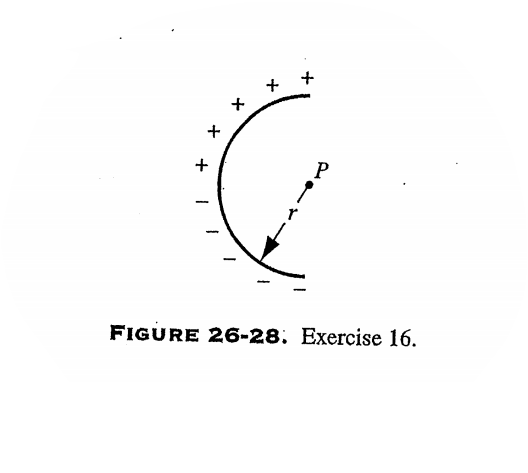
\includegraphics[scale=0.6]{02.png}
  \end{center}
\end{problem}
\begin{solution}
\end{solution}
\newpage

\begin{problem}[26-P2]
Show that the components of $\vec{\mathbf{E}}$ due to a dipole are given, at distant
points, by
\[
  E_x = \f{1}{4\pi\epsilon_0} \f{3pxz}{(x^2+z^2)^{5/2}}, ~~~~~~ E_z = \f{1}{4\pi\epsilon_0} \f{p(2z^2-x^2)}{(x^2+z^2)^{5/2}},
\]
where $x$ and $z$ are coordinates of point $P$ in Fig. 26-37. Show that
this general result includes the special results of Eq. 26-12 and Problem 1.
\begin{center}
  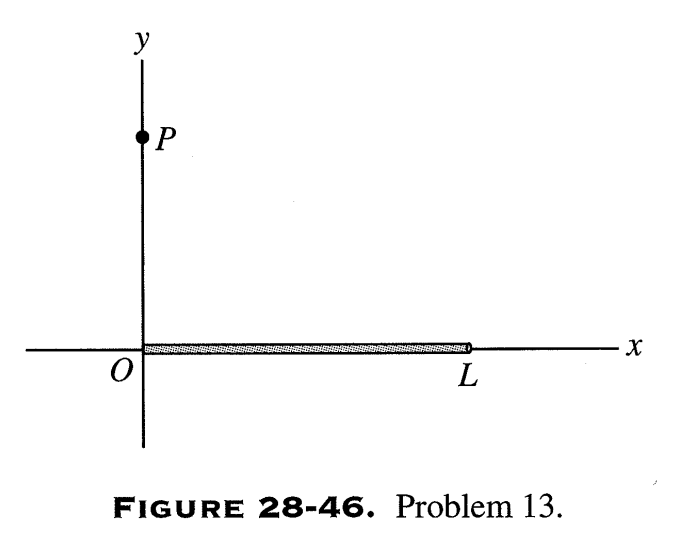
\includegraphics[scale=0.7]{03.png}
\end{center}
\end{problem}
\begin{solution}
\end{solution}
\newpage 

\begin{problem}[25-P7*]
A certain charge $Q$ is to be divided into two parts, $Q-q$ and $q$. What is the relation of $Q$ to $q$ if two parts, placed a given distance apart, are to have a maximum Coulomb repulsion.
\end{problem}
\begin{solution}
\end{solution}

\end{document}
